\chapter{Mechanische Umsetzung}  \label{Mechanische Umsetzung}
\fancyfoot[C]{Schmeisser}

\section{Gehäuse}
\subsection{Anforderung an das Gehäuse}

Da das Grundprodukt eine Ducati S4 Monster 2001 mit Verbrennungsmotor war, musste der Motor entfernt werden, um die benötigten Teile für eine Umrüstung auf E-Antrieb unterbringen zu können. Bei allen Motorrädern ist der Motorblock ein teil des Gehäuses beziehungsweise des Rahmens. Aus diesem Grund musste, statt des Verbrennungsmotors, ein platzsparender Ersatz gefunden werden. Das neue Gehäuse muss also die, bei einer Fahrt, aufkommenden Kräfte und Spannungen aufnehmen können. Die Schraubpunkte, mit denen der Rahmen des Motorrades zuvor zusammengehalten wurde, mussten ebenfalls im selben Bauteil ersetzt werden. Gleichzeitig mussten neue Schraubpunkte für Getriebe, Motor, Akkupacks, und weiteren Komponenten geschaffen werden, da sonst ein sicherer Betrieb nicht möglich wäre. Weiters sollte das neue Gehäuse ein Schlag- und Spritzschutz für die dahinter, im inneren liegenden Bauteile und Komponenten des Motorrades sein. Neben alldem soll natürlich auch der Fahrer nicht mit Körperteilen, oder sonstigen, am Körper anliegenden Gegenständen, in das Getriebe, oder beispielsweise die Motorsteuerung, gelangen können.\\\medskip

\textbf{Zusammenfassend soll der Motorblockersatz folgendes übernehmen:}\\\medskip

\begin{itemize}
	\item Anfallende Kräfte in Normal-, sowie in Unfallsituationen verkraften.
	\item Schraubpunkte des Motorblocks ersetzen, ohne die das Motorrad in sich zusammenfallen würde.
	\item Neue Anschraubpunkte für Bauteile und Getriebe vorsehen.
	\item Schlag- und Spritzschutz für Bauteile und wichtige Komponenten, sowie Schutz für den Fahrer.
\end{itemize}

\newpage

\subsection{Dimensionierung}
Die Dimensionierung richtete sich im Großen und Ganzen nach dem Platzbedarf der Bauteile und dem Gewicht, welches noch belegt werden darf, bis der Grenzwert erreicht ist. Nach der Wahl des Gesamtkonzepts beziehungsweise nachdem feststand, was alles für ein funktionstüchtiges Motorrad benötigt wird, könnte mit der Dimensionierung des Gehäuses begonnen werden. 

\subsection{Gewicht}
Da Die Akku-Zellen mit Abstand das schwerste am neuen Motorrad sind, musste, um nicht die Grenzwerte des vorhergehenden Motorades zu sprengen, der Rest so Gewichtsparend wie möglich geplant werden. Anstatt von Stahl konnte durch Berechnungen auch Aluminium als ausreichendes Material ausfindig gemacht werden. Da Aluminium leichter als Stahl ist, wurde neben Kosten auch Gewicht gespart. 

\subsection{Gesamtgewicht des Zero-Emission-Power-Bikes:}
\begin{table} [H]
	\begin{center}
		\begin{tabular}{|c|c|}
		\hline
		Bezeichnung 						& Gewicht in kg \\ \hline
		Akkuzellen  						& 39,200        \\ \hline
		Akkupacks   						& 3,269         \\ \hline
		Getriebe (ohne Seitenplatte)   	 	& 13,031  		\\ \hline   
		Seitenplatte Links					& 5,067			\\ \hline
		Seitenplatte Rechts					& 5,821			\\ \hline
		BMS									& 1,100			\\ \hline
		Motorsteuerung						& 1,200			\\ \hline
		Akkusteuerung						& 0,700			\\ \hline
		Sonstiges (Schrauben, Leitungen,….) & 2,900			\\ \hline
		Motorrad-Grundgerüst				& 79,000		\\ \hline
		Motor								& 13,000		\\ \hline
		Gesamt								& 164,288		\\ \hline
		\end{tabular}
		\caption{Gewichtstabelle}
	\end{center}
\end{table}


\subsection{Festlegung der Maße}

Nach Absprache mit einigen Lehrern, Maschinenbau-Ingenieuren und dem Projektteam wurde als sinnvollster Ersatz für den Motorblock, zwei Platten ausgewählt. Die Platten enthielten zu Anfang nur die je 3 Bohrungen, als Ersatz für den Rahmen. Mit Fortlauf der Zeit und des Projektes wurden immer mehr Details, vor allem an der Linken Platte vorgenommen. Nach Fertigstellung der Seitenplatten musste das Material und die Stärke ausgewählt werden. Nach einigen Statischen Berechnungen, war eine 20 mm Aluminiumplatte ausreichen für die anfallenden Kräfte. Mit der Entscheidung Aluminiumplatten zu verwenden, konnten Kosten, wie auch Gewicht gespart werden.

\subsection{Material}
\begin{table} [H]
	\begin{center}
		\begin{tabular}{|c|c|}
		\hline
		Aluminiumlegierung:			& 3.3547 ,  AlMg4.5Mn, EN-AW 5083 \\ \hline
		Dichte:						& 2,660 kg/dm		\\ \hline
		Wärmeausdehnungskoeffizien:	& 0,0000 /c			\\ \hline
		Wärmeleitfähigkeit:			& 0,204 kW/m-C		\\ \hline
		Spezifische Wärme:			& 940,000 J/kg-C	\\ \hline
		Elastizitätsmodul:			& 70000,000 MPa		\\ \hline
		Poissonscher Beiwert:		& 0,390				\\ \hline
		Streckgrenze:				& 270,000 MPa		\\ \hline
		Zugfestigkeit:				& 345,000 MPa		\\ \hline
		\end{tabular}
		\caption{Aluminium: AlMg4.5Mn Materialdaten}
	\end{center}
\end{table}


\begin{figure} [H]
	\begin{center}
		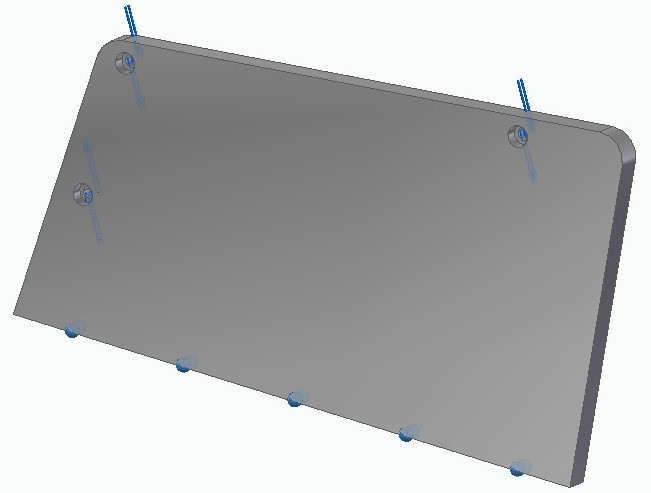
\includegraphics[scale=0.5]{figures/mechanik/Seitenplatte_Rechts.jpg}
			\caption{Seitenplatte Rechts}
			\label{fig:Seitenplatte Rechts}
	\end{center}
\end{figure}

\begin{figure} [H]
	\begin{center}
		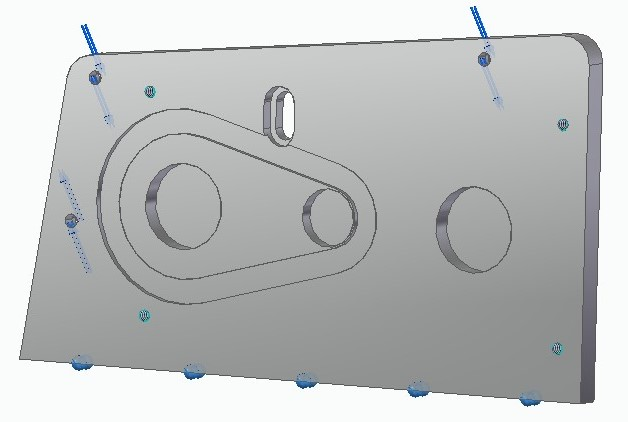
\includegraphics[scale=0.5]{figures/mechanik/Seitenplatte_Links_innen.jpg}
			\caption{Seitenplatte Links Innenansicht}
			\label{fig:Seitenplatte Links Innenansicht}
	\end{center}
\end{figure}

Neben den Platten, waren noch weitere kleinere Gehäuseteile nötig um den Rahmen neu in Betrieb zu nehmen. Dabei handelt es sich um den Achsenersatz für den Schwingarm, an dem das Hinterrad angebracht ist. 

\begin{figure} [H]
	\begin{center}
		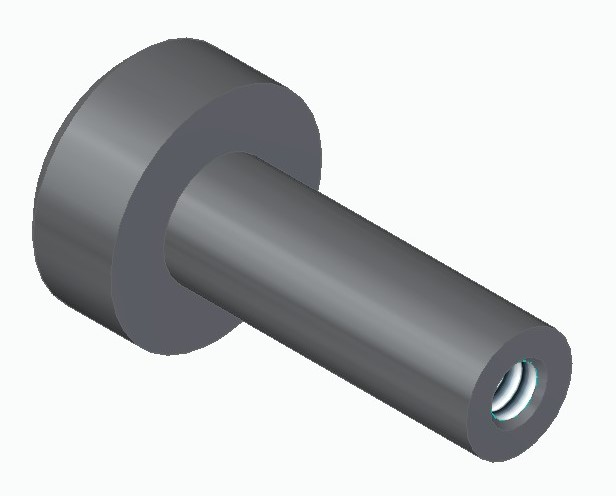
\includegraphics[scale=0.2]{figures/mechanik/Welle_Rechts.jpg}
			\caption{Wellenersatz}
			\label{fig:Wellenersatz}
	\end{center}
\end{figure}

\newpage

\section{Getriebe}

\subsection{Aufgabe des Getriebes}

Durch die hohen Umdrehungswerte des Elektromotors musste ein Getriebe diese herunterwandeln, weil ansonsten beim Start ein zu geringes Drehmoment vorhanden gewesen wäre und bei maximaler Drehzahl, eine theoretische Geschwindigkeit von gerundet 300 km/h, das Ergebnis gewesen wäre. Im Projekt wurde dieses Getriebe mit einem Kettengetriebe realisiert um ein Zahnradgetriebe zu vermeiden. Der Grund dafür wird unten näher erläutert.

\subsection{Das Getriebe}

Bei dem Getriebe wurde entschieden, dass kein Zahnradgetriebe verwendete werden wird, da ein solches in Öl getränkt sein muss und dafür die Getriebebox vollständig wasserdicht sein müsste. Stattdessen wurde ein Kettengetriebe als ausreichend empfunden. 
Nach reichlicher Recherche wurde klar, dass nicht nur eine zusätzliche Kette, sondern sogar zwei zusätzliche Ketten notwendig waren um ein Übertragungsverhältnis von 1: 9,25  zu erhalten. Die Zahnräder wären aufgrund der großen Drehmomente, der hohen Anzahl an Zähnen und des damit verbundenen Durchmessers zu groß gewesen. Somit entstand ein Fahrwerk mit insgesamt drei Ketten, sechs Kettenrädern und 2 Kettenspannern. 
Bei den Kettenrädern, sowie auch bei der Kette musste der Platzbedarf zu den auftretenden Kräften abgewogen werden. Die originale Kette ist eine aus der Normreihe B-1 10. Da aber in dieser Norm die Zahnräder größer sind, um größeren Kräften standhalten zu können, hätte ein größeres Getriebe eingeplant werden müssen. Nach Berechnungen könnte eine kleinere Norm ebenfalls als ausreichend befunden werden. Die maximalen Drehmomente in der Norm B-1 08, sind immer noch ausreichen für Extrem- und Alltagssituationen. Mit dieser Erkenntnis könnte wieder einiges an Platz gespart werden.

\newpage

\begin{figure} [H]
	\begin{center}
		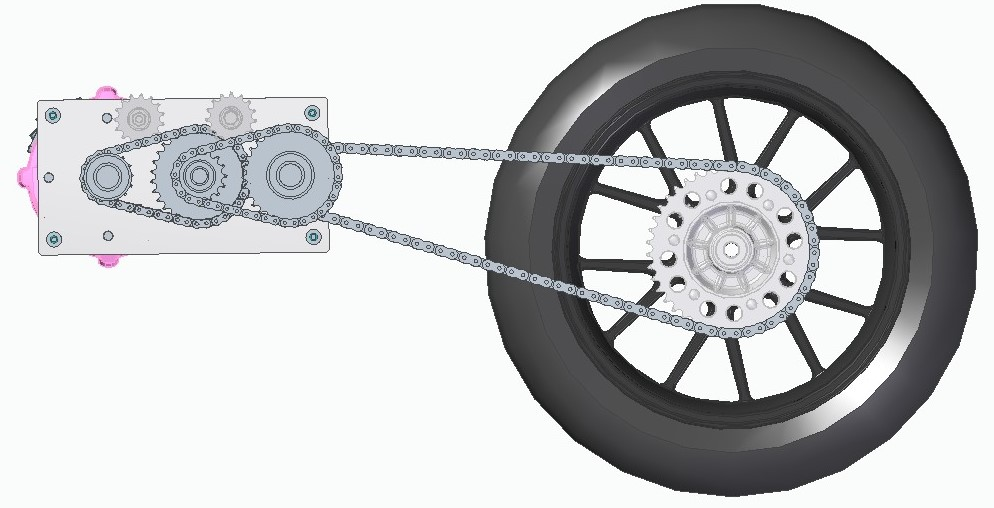
\includegraphics[scale=0.5]{figures/mechanik/Getriebe.jpg}
			\caption{Getriebeansicht Seitlich}
			\label{fig:Getriebeansicht Seitlich}
	\end{center}
\end{figure}






\begin{figure} [H]
	\begin{center}
		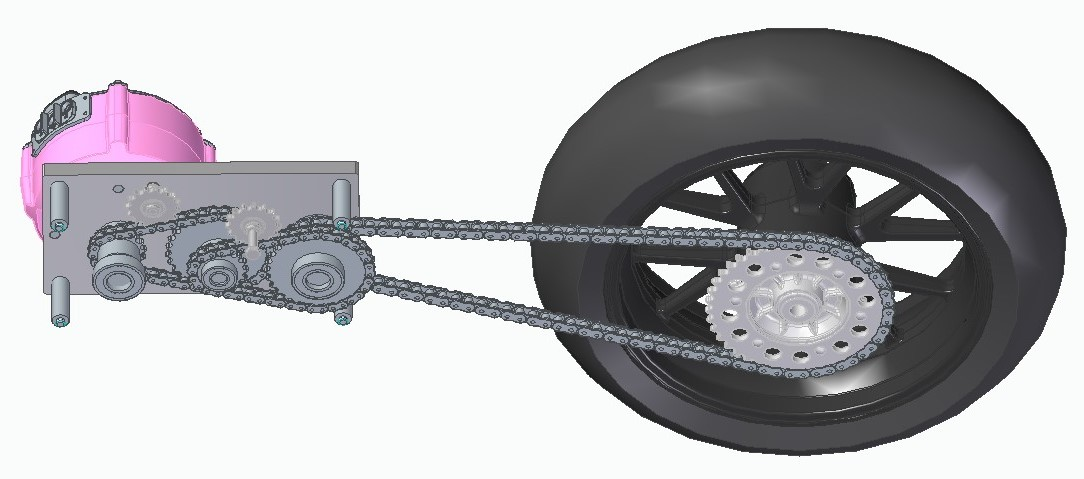
\includegraphics[scale=0.5]{figures/mechanik/Getriebe_2.jpg}
			\caption{Getriebeansicht Schräg}
			\label{fig:Getriebeansicht Schräg}
	\end{center}
\end{figure}

\newpage

\subsection*{Einzelteile}

Die Zahnräder sind auf insgesamt 3 Achsen montiert, welche die Kraft von einem Kettenrad zum nächsten übertragen soll. Um dies zu gewährleisten, werden diese aus Stahl gefertigt, um das Risiko eines Reißens der Achse zu vermeiden. Die Zahnräder werden mit Passfedern und Schrauben an die Achse gepresst. Die Achsen sind Kugelgelagert in der linken Seitenplatte und der Aufbauplatte versenkt.

\subsubsection*{Achse 1 / Antriebsachse}

Achse 1/Antriebsachse :	Verbindet die Motorwelle mit dem ersten Zahnrad (15 Zähne B-1 08). Am anderen Ende befindet sich ein Kugellager.

\begin{figure} [H]
	\begin{center}
		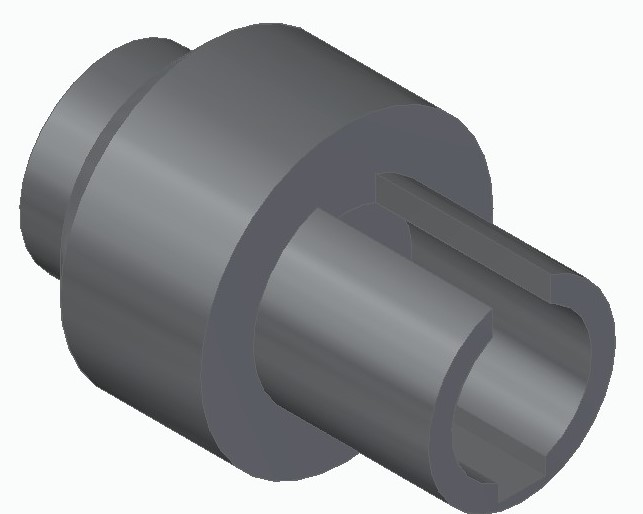
\includegraphics[scale=0.4]{figures/mechanik/Antriebsachse.jpg}
			\caption{Achse 1/Antriebsachse}
			\label{fig:Achse 1/Antriebsachse}
	\end{center}
\end{figure}

\subsubsection*{Achse 2}

Am größerem Zylinder sitzt ein Zahnrad mit 30 Zähnen (B-1 08), welches mittels einer Kette mit dem ersten Zahnrad (15 Zähne B-1 08) von der 1. Achse verbunden ist. Über die Achse wird das Drehmoment und die Drehzahl auf das Nächste Zahnrad (16 Zähne B-1 08) übertragen. An beiden Enden ist jeweiles ein Kugellager, wobei auf der rechten Seite, von dieser Perspektive aus gesehen, ein kleineres notwendig war, um den Kettenverlauf des Zahnrades nicht zu behindern. (Eine genauere Erklärung folgt.)

\begin{figure} [H]
	\begin{center}
		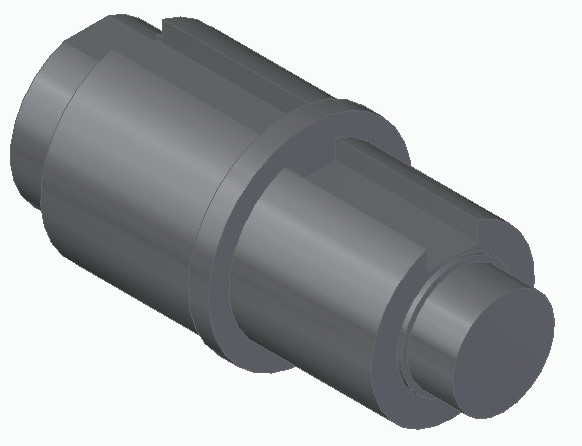
\includegraphics[scale=0.5]{figures/mechanik/Achse_mit_nuten_20mm.jpg}
			\caption{Achse 2}
			\label{fig:Achse 2}
	\end{center}
\end{figure}

\subsubsection*{Achse 3}

Dies ist die letzte Achse, bevor das Hinterrad angetrieben wird. Am größeren Zylinder befindet sich wieder ein 30-zähniges Kettenrad der Norm B-1 08 und am kleineren Zylinder ein 15-zähniges Zahnrad der Norm B-1 10. Bei dem Kettenrad mit 30 Zähnen war ein Eingriff in die Norm-Bauform notwendig, um die Antriebskette nicht zu blockieren (Eine genauere Erklärung später). An beiden Seiten der Achse befindet sich jewils ein Kugellager der selben Bauform. 


\begin{figure} [H]
	\begin{center}
		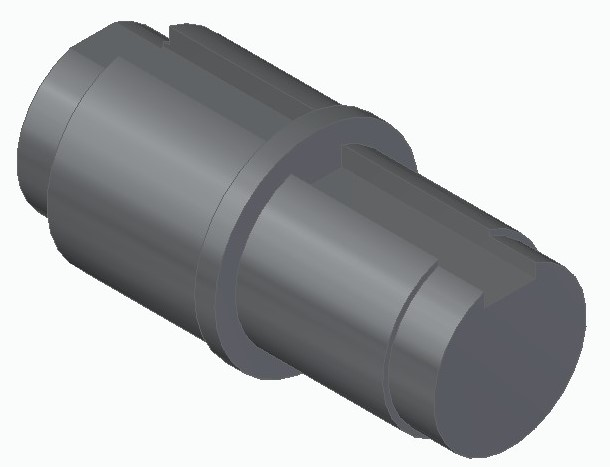
\includegraphics[scale=0.5]{figures/mechanik/Achse_mit_nuten.jpg}
			\caption{Achse 3}
			\label{fig:Achse 3}
	\end{center}
\end{figure}

\subsubsection*{Getriebegegenplatte und Abstandhalter}

Für das Getriebe war, wie schon erwähnt, eine Gegenplatte notwendig. An diese Platte wird auch der Motor und das mittlere Akkupack befestigt. Mit 4 Schrauben und dazugehörigen Abstandhalter wird das Getriebe zusammengehalten. Die Abstandhalter sind 4 Stahlrohre mit Innendurchmesser 10 mm und Außendurchmesser 20 mm.

\begin{figure} [H]
	\begin{center}
		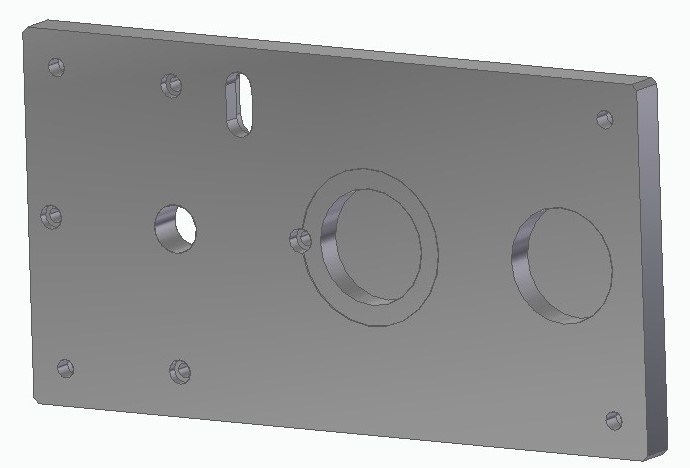
\includegraphics[scale=0.5]{figures/mechanik/Aufbau_Seitenplatte_Links.jpg}
			\caption{Getriebegegenplatte}
			\label{Getriebegegenplatte}
	\end{center}
\end{figure}

\begin{figure} [H]
	\begin{center}
		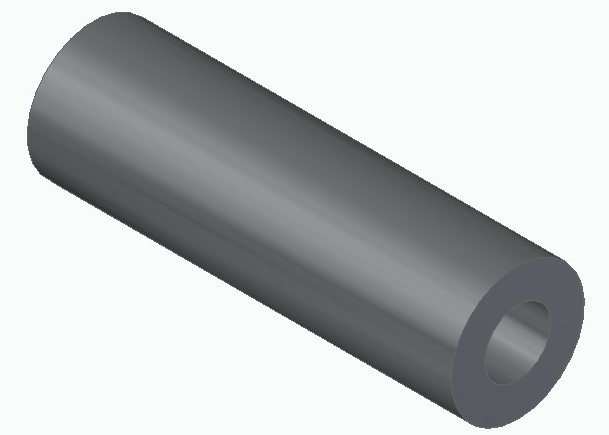
\includegraphics[scale=0.3]{figures/mechanik/Seitenplatte_Abstandhalter.jpg}
			\caption{Abstandhalter}
			\label{Abstandhalter}
	\end{center}
\end{figure}

\subsubsection*{Kettenspanner}

Wenn Ketten zu schwingen beginnen, werden diese sehr schnell kaputt und beeinträchtigen das Fahrverhalten. Um diese Problem zu lösen werden bei Kettenantrieben immer Spannräder benötigt. Bei den ersten beiden Ketten, vom Motor ausgehend, ist jeweils eines vorhanden. Bei der letzten Kette kann diese am Anschraubpunkt der Hinterachse gespannt oder entspannt werden und deshalb ist kein Spannrad notwendig. Die beiden Kettenräder haben 15 Zähne und stammen aus der Norm B-1 08. Die beiden Spannnräder werden mittels einer Außensechskantschraube M16 und 3 Muttern M16 befestigt. Das, vom Motor aus, erste Kettenrad ist an der Aufbauplatte montiert, dort wo auch der Motor befestigt ist. Das zweite Kettenrad ist auf der Seitenplatte befestigt.  Für die Befestigung sind an beiden Platten Nuten eingefräst.


\begin{figure} [H]
	\begin{center}
		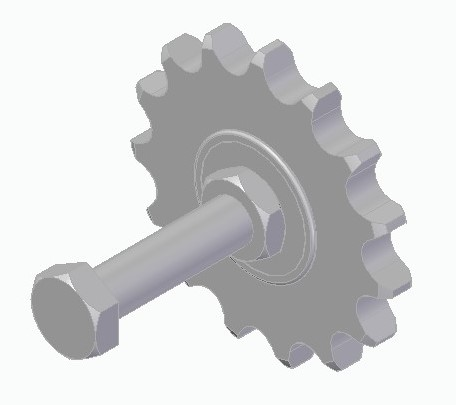
\includegraphics[scale=0.3]{figures/mechanik/14099505.jpg}
			\caption{Kettenspanner}
			\label{fig:Kettenspanner}
	\end{center}
\end{figure}

\newpage

\subsubsection*{Kettenräder}

Das Getriebe umfasst insgesamt fünf Kettenräder (ohne Antriebskettenrad an der Hinterachse) mit verschiedenen Größen, Bezogen auf die Anzahl der Zähne, aus zwei verschiedenen Normen, um das Getriebe mit an die originale Kette anpassen zu können: 

\subsection*{ISO 08 B-1 Teilung 1/2 x 5/16"}

\begin{figure} [H]
	\begin{center}
		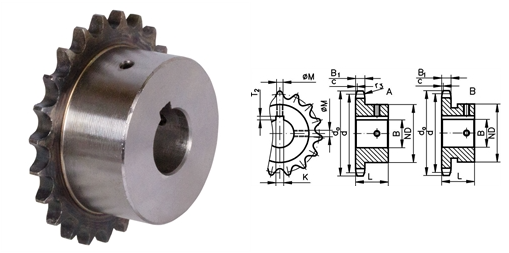
\includegraphics[scale=0.7]{figures/mechanik/ISO 08 B-1 .PNG}
			\caption{ISO 08 B-1}
			\label{fig:ISO 08 B-1}
	\end{center}
\end{figure}

Werkstoff: Stahl C45. Zähne gefräst und induktiv gehärtet (ca. HRC 50). Einbaufertig, für diverse Wellendurchmesser. Fertigbohrung H7 -Rauwert Ra 1,6, Nut nach DIN 6885/1 auf Zahnspitze ausgerichtet, 2 Stellschraubengewinde, einmal auf Nut ausgerichtet, einmal 90° versetzt. Allgemeine Abmessungen: B1 = 7,2 mm, c = 1,3 mm, r3 = 13 mm. 
Weiter Daten sind aus der folgenden Tabelle zu entnehmen.

\begin{table}[H]
	\begin{tabular}{|c|c|c|c|c|c|c|c|c|c|c|c|}
	\hline
		\textbf{Produkt} & \textbf{Zähne} & \textbf{B H7} & \textbf{Type} & \textbf{da} & \textbf{d} & \textbf{ND} & \textbf{L} & \textbf{KH9} & \textbf{T2} & \textbf{M} & \textbf{Gewicht} \\ \hline
		                 & \textbf{}                 & mm                           &               & mm          & mm         & mm          & mm         & mm           & mm          &            & kg               \\ \hline
		10681532         & 15                        & 32                           & B             & 65,5        & 61,09      & 49          & 28         & 10           & 3,3         & M8         & 0,300            \\ \hline
		10581632         & 16                        & 32                           & A             & 69,5        & 65,10      & 53          & 28         & 10           & 3,3         & M8         & 0,334            \\ \hline
		10583038         & 30                        & 38                           & A             & 126,1       & 121,50     & 80          & 30         & 10           & 3,3         & M8         & 1,219            \\ \hline
	\end{tabular}
	\caption{Auszug Wertetabelle ISO 08 B-1}
\end{table}

\newpage

\subsection*{ISO 10 B-1 Teilung 5/8 x 3/8"}

\begin{figure} [H]
	\begin{center}
		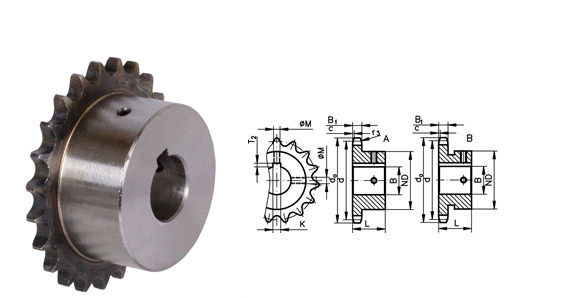
\includegraphics[scale=0.7]{figures/mechanik/ISO 10 B-1 .PNG}
			\caption{ISO 10 B-1}
			\label{fig:ISO 10 B-1}
	\end{center}
\end{figure}

Werkstoff: Stahl C45. Zähne gefräst und induktiv gehärtet (ca. HRC 50). Einbaufertig, für diverse Wellendurchmesser. Fertigbohrung H7 -Rauwert Ra 1,6, Nut nach DIN 6885/1 auf Zahnspitze ausgerichtet, 2 Stellschraubengewinde, einmal auf Nut ausgerichtet, einmal 90° versetzt. Allgemeine Abmessungen: B1 = 9,1 mm, c = 1,6 mm, r3 = 16 mm. 
Weiter Daten sind aus der folgenden Tabelle zu entnehmen.

\begin{table}[H]
\begin{tabular}{|c|c|c|c|c|c|c|c|c|c|c|c|}
\hline
\textbf{Produkt} & \textbf{Zähne} & \textbf{B H7} & \textbf{Type} & \textbf{da} & \textbf{d} & \textbf{ND} & \textbf{L} & \textbf{KH9} & \textbf{T2} & \textbf{M} & \textbf{Gewicht} \\ \hline
                 & \textbf{}                 & mm                           &               & mm          & mm         & mm          & mm         & mm           & mm          &            & kg               \\ \hline
10681532         & 15                        & 32                           & B             & 83,0        & 76,36      & 57          & 30         & 8            & 3,3         & M6         & 0,501            \\ \hline
\end{tabular}
\caption{Auszug Wertetabelle ISO 10 B-1}
\end{table}

\newpage

\begin{figure} [H]
	\begin{center}
		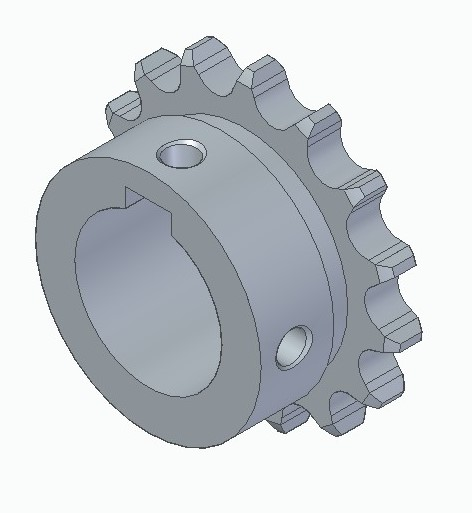
\includegraphics[scale=0.3]{figures/mechanik/10581532.jpg}
			\caption{Kettenrad Z=15 B-1 08}
			\label{fig:Kettenrad Z=15 B-1 08}
	\end{center}
\end{figure}


\begin{figure} [H]
	\begin{center}
		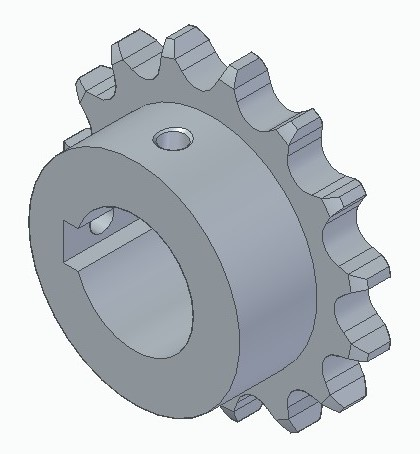
\includegraphics[scale=0.3]{figures/mechanik/10681532.jpg}
			\caption{Kettenrad Z=15 B-1 10}
			\label{fig:Kettenrad Z=15 B-1 10}
	\end{center}
\end{figure}


\begin{figure} [H]
	\begin{center}
		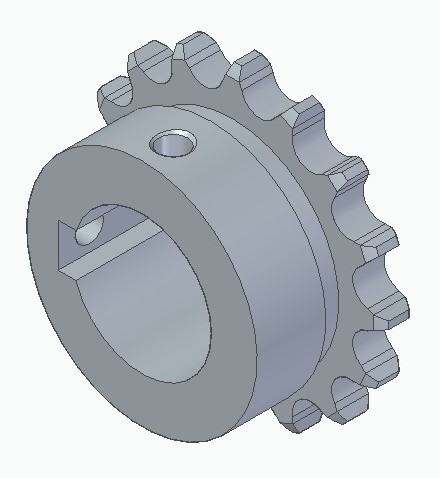
\includegraphics[scale=0.3]{figures/mechanik/10581632.jpg}
			\caption{Kettenrad Z=16 B-1 08}
			\label{fig:Kettenrad Z=16 B-1 08}
	\end{center}
\end{figure}


\begin{figure} [H]
	\begin{center}
		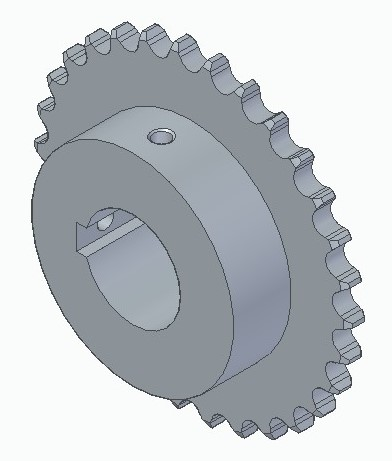
\includegraphics[scale=0.3]{figures/mechanik/10583038.jpg}
			\caption{Kettenrad Z=30 B-1 08}
			\label{fig:Kettenrad Z=30 B-1 08}
	\end{center}
\end{figure}


\begin{figure} [H]
	\begin{center}
		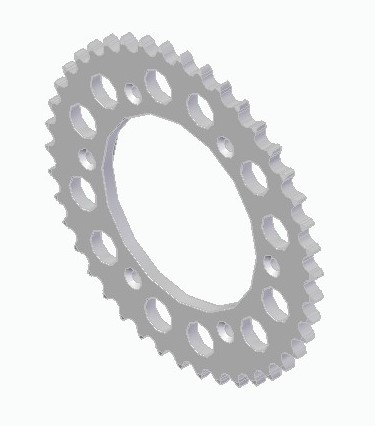
\includegraphics[scale=0.3]{figures/mechanik/2000 Monster M750 swingarm, suspension.jpg}
			\caption{Ducati Kettenrad Z=37 B-1 10}
			\label{fig:Ducati Kettenrad Z=37 B-1 10}
	\end{center}
\end{figure}

\newpage

\subsubsection*{Kugellager}

Kugellager: Innendurchmesser 20 mm Außendurchmesser 42 mm Stärke 12 mm
\begin{figure} [H]
	\begin{center}
		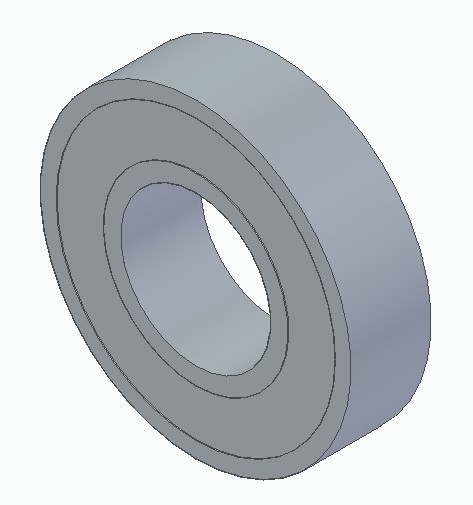
\includegraphics[scale=0.3]{figures/mechanik/6004-2RSH-SKF_gr.jpg}
			\caption{Kugellager 1}
			\label{fig:Kugellager 1}
	\end{center}
\end{figure}

 
Kugellager: Innendurchmesser 30 mm Außendurchmesser 62 mm Stärke 16 mm
\begin{figure} [H]
	\begin{center}
		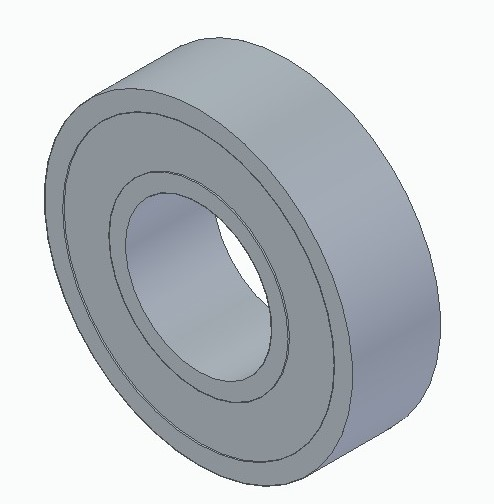
\includegraphics[scale=0.3]{figures/mechanik/6206-2RS1-SKF_kl.jpg}
			\caption{Kugellager 2}
			\label{fig:Kugellager 2}
	\end{center}
\end{figure}

Vor Beginn der Planung, muss die Verfügbarkeit der Bauteile, durch Lieferanten und Firmen sichergestellt werden. Nach fixer Zusage von Lieferanten sowie verschiedenen Firmen wurde das Getriebe unter Hochdruck geplant. Da im Getriebe sehr hohe Kräfte aufkommen, muss garantiert sein, dass alles in der Genauigkeit eines Hundertstelmillimeter passt. Ebenfalls dürfen die Zahnräder nicht an Seitenplatten anstoßen oder streifen, weil ein enorm hoher Verschleiß die Folge wäre. 

Das Getriebe ist eine Spezialanfertigung, welches für diese Projekt erstellt wurde. Alle Abstände von Zahnrad zu Zahnrad, sind so klein wie möglich. Die Befestigungspunkte für den Aufbau, sind ebenfalls mit dem geringsten Abstand zu den Kettenrädern angebracht. Durch sämtliche Optimierungen konnte Geld für das Material und Gewicht für das Motorrad gespart und dennoch ein sicherer Betrieb ermöglicht werden.

\newpage

\subsection*{Seitenplatte mit Getriebe-Fräsungen}

Diese ist die komplizierteste Platte bei diesem Projekt. Wie die rechte Seitenplatte, enthält diese auch die drei Bohrungen für die Rahmen- und Schwingarmaufhängung. Aber unter anderem ist diese auch Teil des Getriebes. Das Getriebe ist ausschließlich auf dieser Platte aufgehängt und trägt somit auch den Motor und einen Teil des mittleren Akkus. 
Es war ein Mittelweg zu finden, der es ermöglicht Kugellager, welche die Achsen beinhalten, Form-Fräsungen für den Verlauf von Ketten, weitere zusätzliche Bohrungen zu erstellen und noch die erforderliche Festigkeit für den Motorblock zu erhalten. Mit jeder Entfernung von Material vom Bauteil, wird seine Festigkeit verringert und damit die Gefahr eines Zusammenbruchs größer.
Dieses Bauteil erforderte große Sorgfalt und genaue Planung um all dies zu vermeiden.
Berechnungen (siehe Anhang).   


\subsection*{Problemstellung des Getriebes}

Wie oben schon erwähnt, musste eines der beiden 30-Zahn-Kettenräder bearbeitet werden. Wie im Bild zu sehen, würde ohne Bearbeitung die Kette zerstört werden, beziehungsweise würde das Getriebe nicht funktionieren. Es muss ein kleiner Teil weggedreht werden, um einen fehlerfreien Betrieb gewährleisten zu können.


\begin{figure} [H]
	\begin{center}
		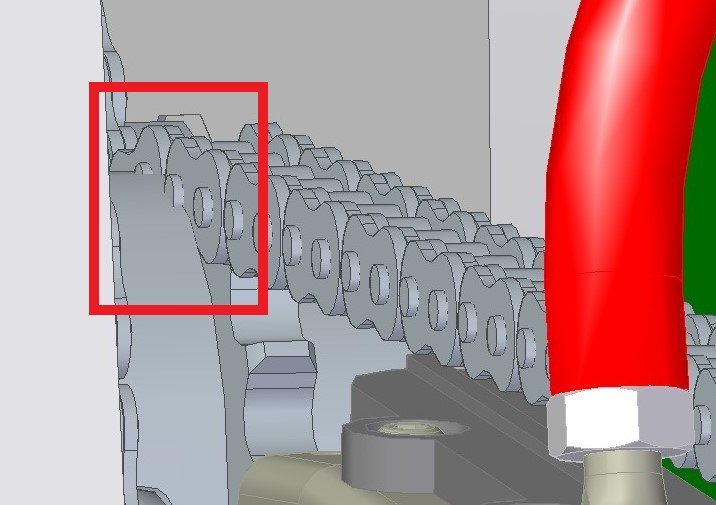
\includegraphics[scale=0.5]{figures/mechanik/Getriebeproblem2.jpg}
			\caption{Getriebeproblem 1}
			\label{fig:Getriebeproblem 1}
	\end{center}
\end{figure}

Das zweite Problem war aufgrund eines Kugellagers, welches das selbe Problem zur Folge hätte, wie bei dem Kettenrad von oben. Die Lösung war ein kleineres Kugellager, welches einen kleineren Durchmesser hat, die Zahnscheibe des Kettenrades.

\begin{figure} [H]
	\begin{center}
		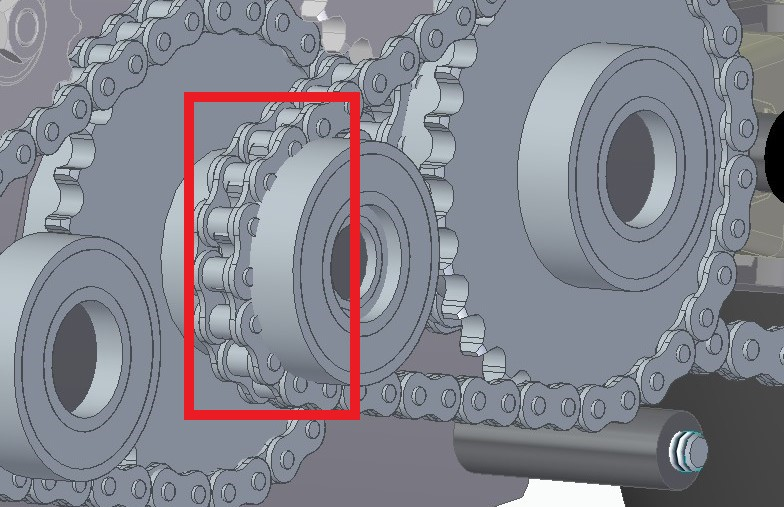
\includegraphics[scale=0.5]{figures/mechanik/Getriebeproblem1.jpg}
			\caption{Getriebeproblem 2}
			\label{fig:Getriebeproblem 2}
	\end{center}
\end{figure}

\newpage

\section{Akkupacks}
Als am besten geeignetes Material für die Packs ergab sich Polycarbonat. Dieses Material lässt sich verkleben und zurechtschneiden, ist dann aber doch nahezu unzerstörbar. Mit 6 mm Stärke ist das für dieses Projekt ausgewählte Material Schlagsicher. Mit 8 mm währe es schon kugelsicher. Zudem wiegen dies Platten auch nicht sehr viel und sind daher ein perfektes Material.
Die Packs sind so entworfen, dass sich ein Vielfaches von 40 Zellen einfach zusammenschließen lässt. Neben den Akkus muss natürlich auch eine Kühlmöglichkeit Platz finden. Das Design ist zu erst einmal darauf ausgelegt, dass so viele Zellen wie nur möglich in den Packs Platz haben, sportliches Aussehen oder Design ist zweitranig.

\subsection{Akkupack Vorderseite}
Die vordere Akkubox beinhaltet 240 Akkuzellen. Das Design richtet sich ein wenig nach der Originalform der Ducati S4 und bildet einen Übergang auf die Seitenplatten. Befestigt wird diese Box mit Schrauben nach oben weg. Die Steuerbox und eine Weitere Platte bilden ein Gegenstück für Schrauben. Um Sicher gehen zu können wird die Box noch von einem Metalgurt, der unten um dem Körper führt, welcher dann am Rahmen befestigt wird. Die Verbindung von Akku zur Akku- und Motorsteuerung wird mit Leitungen ermöglicht. Damit die Bohrungen für die Leitungen keine undichte Stelle wird, wird hier eine Kabelverschraubung verwendet um die Stelle abzudichten.


\begin{figure} [H]
	\begin{center}
		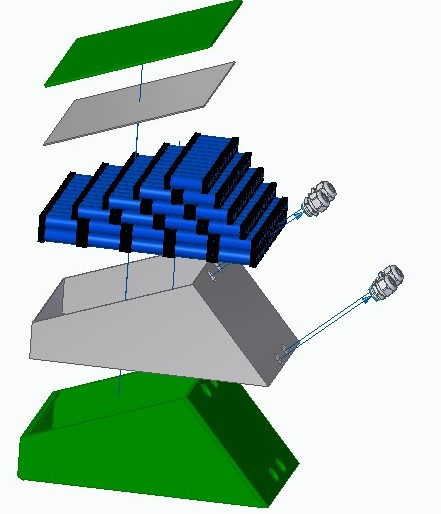
\includegraphics[scale=0.5]{figures/mechanik/Akku_Unterseite_Explosion.jpg}
			\caption{Akku Vorderseite}
			\label{fig:Akku Vorderseite}
	\end{center}
\end{figure}

\newpage

\subsection{Akkupack Motorblock}
Die große Akkubox in der Mitte beinhaltet 220 Akkuzellen, also um 20 zu wenig, oder zu viel. Diese 20 Zellen werden mit 20 Zellen aus der oberen liegenden Box verbunden um die gewünschte Spannung zu erreichen. Dieses Akkupack ist in den Freiraum zwischen den beiden Platten (Rechte Seitenplatte und Aufbauplatte vom Getriebe) und dem Motor eingepasst. Dieser Akku wird dann mit Schrauben an der linken und rechten Seite befestigt. Damit eine Verbindung zu dem vorderem Akku geschaffen werden kann, ist auch hier eine Kabelverschraubung notwendig, durch die, die Leitung verlaufen soll. 


\begin{figure} [H]
	\begin{center}
		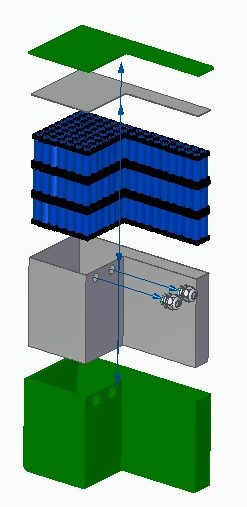
\includegraphics[scale=0.5]{figures/mechanik/Akku_Motorblock_Explosion.jpg}
			\caption{Akku Motorblock}
			\label{fig:Akku Motorblock}
	\end{center}
\end{figure}


\subsection{Akkupack Mitte}
Die kleine Akkubox in der Mitte des Motorrades, direkt unter dem Sitz, beinhaltet die oben schon erwähnten fehlenden 20 Zellen des großen Akkupacks und den Rest auf die Endsumme von 560 Zellen. Diese Box ist im Rahmen so eingepasst, dass der Platz am besten genützt ist und der Stoßdämpfer, vom Schwingarm die Box nicht beschädigt. Die Verbindung vom oberen zum unteren Pack wird mit einer Bohrung hergestellt. Weil diese beiden Boxen gemeinsam verschraubt werden, müssen keine weiteren Dichtungsmaßnahmen vorgesehen werden.


\begin{figure} [H]
	\begin{center}
		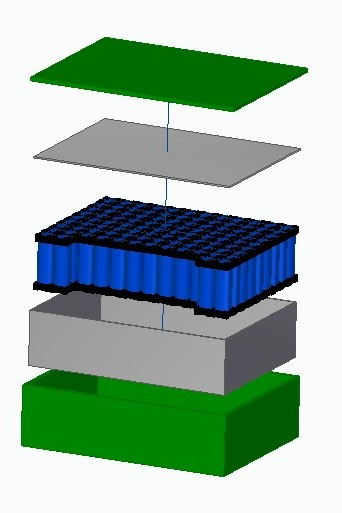
\includegraphics[scale=0.5]{figures/mechanik/Akku_Mitte_Explosion.jpg}
			\caption{Akku Mitte}
			\label{fig:Akku Mitte}
	\end{center}
\end{figure}

\newpage

\section{Akkukühlung}  \label{Akkukühlung}

Für den Prototypen, wurde das Kühlsystem so einfach, wie nur möglich gestaltet. Die ohnehin zu geringe Zeitvorgabe, war der Grund, warum eine Wärmeübertragungskühlung gewählt wurde. Diese Kühlungsmethode entspricht in etwa dem der Peltier-Elemente. 
Im Inneren der Akkupacks sind die Wände mit Aluminiumplatten ausgekleidet. Zusätzlich sind noch Platten mitten hindurch eingeplant, die verschiedene Teile des gesamten Packs unterteilen. Sämtliche Aluminiumplatten, sind thermisch und somit auch elektrisch, miteinander verbunden. Mithilfe von Leitfähigen Leitern, werden diese Kühlungen mit Teilen außerhalb des Akkus verbunden. 
Teile, die am Motorrad angebracht sind, werden vom Fahrtwind umströmt und dadurch gekühlt. 
Dieser Effekt, wird bei diesem System ausgenützt. Die Wärmeenergie der Akkuzellen, soll also an die Umgebung abgegeben werden.
Bei zukünftigen Modellen, wird ein Flüssigkeitssystem in Form einer Wasserkühlung verwendet werden, um die bestmögliche Kühlung gewährleisten zu können.

Siehe Akkukühlung im Motorblock-Pack

Siehe Akkukühlung im Mittel-Pack

Siehe Akkukühlung im Vorderseiten-Pack

\subsection{Warum eine Kühlung notwendig ist}

Wenn ein Akku eine gewisse Größe erreicht, muss dieser gekühlt werden, um nicht zu überhitzen. Wenn eine Akkuzelle Leistung abgibt, erwärmt sich diese. Die logische Schlussfolgerung ist nun, je mehr Akkuzellen vorhanden sind, desto größer ist die Erwärmung in diesem Raum. Es würde mit dem Fahrtwind eine Luftkühlung völlig ausreichend sein, nur die Packs sind in Boxen untergebracht. Durch die zusätzliche Hülle, um die Zellen vor Wasser, Steinschlag, oder Ähnlichem zu schützen, kann eine Luftkühlung nicht realisiert werden. Gleichzeitig wirkt die Box wie eine Isolierung, wodurch sich die Packs immer schneller erhitzen.
Wenn nun keine Kühlung verwendet wird, erhitzt sich das Innere so lange, bis sich sämtliche Zellen aufzulösen beginnen. Das Polycarbonat würde extrem beansprucht werden. Wenn die Zellen immer weiter Leistung abgeben, kommt es bei Lithium-Ionen-Zellen schlussendlich zu einer Explosion.  
Gegen solche Fälle ist im Betriebssystem ein Warnsystem vorhanden. Ebenfalls sind Schutzeinrichtungen wie Sicherungen eingebaut, die ein solches Szenario verhindern sollen. 
Weil keine 100 prozentige Sicherheit für alle Fälle besteht, ist das Material, wie oben schon erwähnt, ebenfalls auf Extremsituationen ausgelegt und kann die Wärmeentwicklung für einen kleinen Zeitraum standhalten, um im schlimmsten Fall ein Entfernen vom Motorrad zu ermöglichen.

\newpage

\section{Zusammenbau}

Die beiden Seitenplatten, sind mit jeweils 3 Sechskantschrauben mit Rahmen und dem Schwingarm verbunden. Die Schrauben werden mit Sicherheitsmuttern und einer Zulegscheibe festgeschraubt. Bei dem Ersatzteil für die Welle, ist ein Gewinde integriert.



\begin{figure} [H]
	\begin{center}
		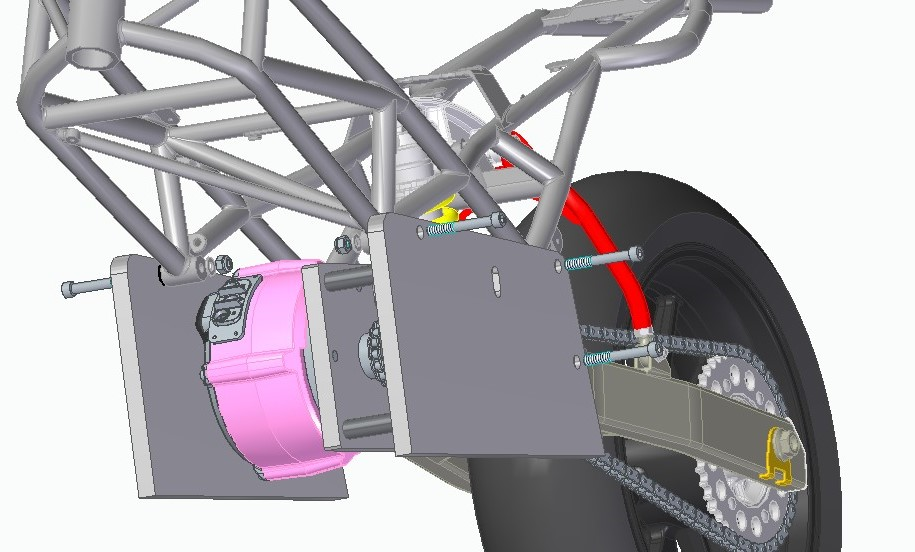
\includegraphics[scale=0.5]{figures/mechanik/Zusamenbau_1.jpg}
			\caption{Befestigung der Seitenplatten}
			\label{fig:Befestigung der Seitenplatten}
	\end{center}
\end{figure}


\begin{figure} [H]
	\begin{center}
		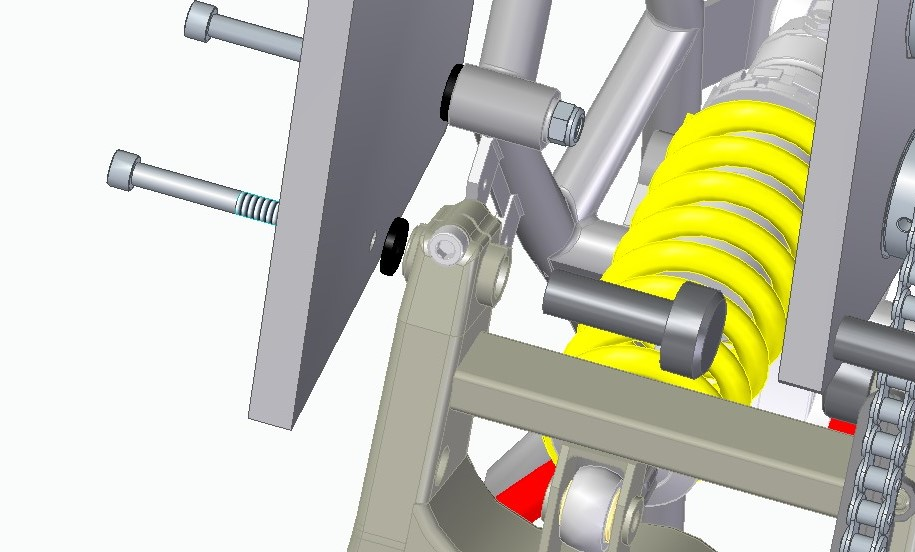
\includegraphics[scale=0.5]{figures/mechanik/Zusammenbau_Schwingarm.jpg}
			\caption{Befestigung des Schwingarmes}
			\label{fig:Befestigung des Schwingarmes}
	\end{center}
\end{figure}

\newpage

In den folgenden Bildern ist das Getriebe mit all seinen Einzelteilen abgebildet. 
In der Mitte die drei Achsen. Jeweils zwei beziehungsweise ein Kettenrad links und rechts der Achsen und zwischen den Kettenrädern und den beiden Aluminiumplatten noch Kugellager.
sämtliche Schrauben, die das Getriebe zusammenhalten sollen, sind auch sichtbar gemacht worden.


\begin{figure} [H]
	\begin{center}
		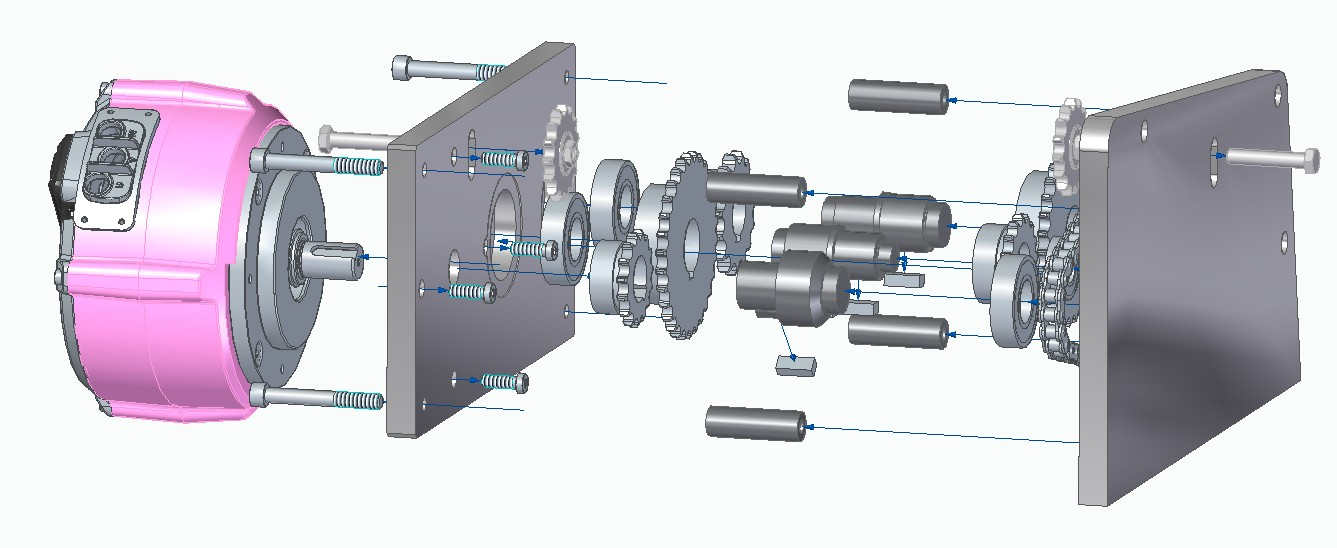
\includegraphics[scale=0.4]{figures/mechanik/Getriebe_Explosion_4.jpg}
			\caption{Explosionsansicht des gesamten Getriebes}
			\label{fig:Explosionsansicht des gesamten Getriebes}
	\end{center}
\end{figure}


\begin{figure} [H]
	\begin{center}
		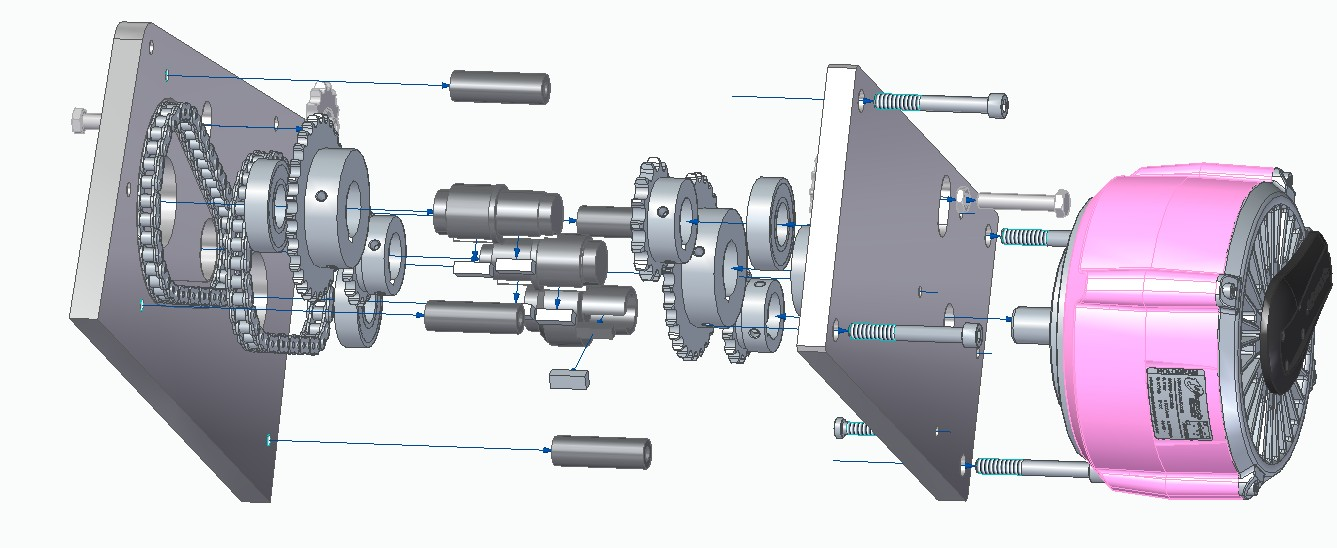
\includegraphics[scale=0.4]{figures/mechanik/Getriebe_Explosion_5.jpg}
			\caption{Detailansicht Getriebe}
			\label{fig:Detailansicht Getriebe}
	\end{center}
\end{figure}



 
%Akku mitte ist in Abbildung \ref{fig:akkuMitte} und ist auf Seite \pageref{fig:akkuMitte}
%
%
%\begin{figure} [H]
%	\begin{center}
%		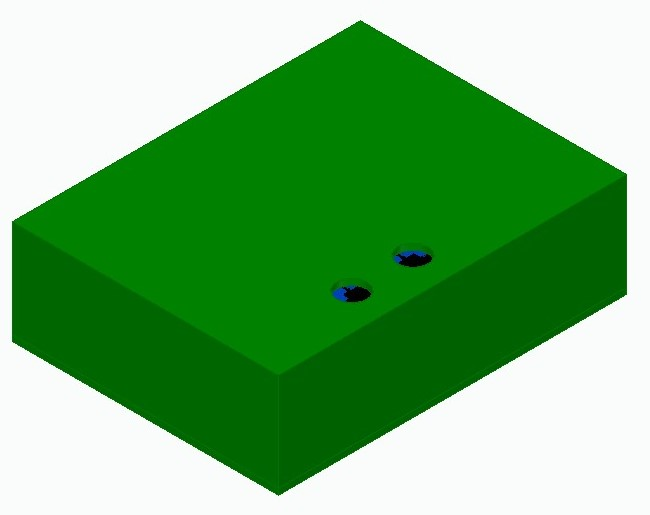
\includegraphics[scale=0.5]{figures/mechanik/Akku_Mitte.jpg}
%			\caption{Akku Mitte}
%			\label{fig:akkuMitte}
%	\end{center}
%\end{figure}
%
%\begin{table} [H]
%	\begin{center}
%		\begin{tabular}{|c|c|}
%		\hline
%		Bezeichnung & Gewicht in kg \\ \hline
%		Akkuzellen  & 39,200        \\ \hline
%		Akkupacks   & 3,269         \\ \hline
%		Getriebe    & 13,031  		\\ \hline   
%		\end{tabular}
%		\caption{Gewichtstabelle}
%	\end{center}
%\end{table}